\section{Module 85: Register Allocation}
\begin{flushright}
\textit{(scribed by Jai Javeria)}
\end{flushright}
The Intermediate Representation uses an unlimited number of temporaries. While this simplified code generation and optimization, a machine only has  finite resources and thus we need to map potentially large number of temporaries with the machine registers.

\subsection{Many to One Mapping}
\begin{itemize}
    \item Since there are more temporaries than registers, we would have to assign multiple temporaries to a single register without changing program behavior. 
    \item If this is not possible then we have to store('spill') some of the temporaries in the memory.
    \item We can have a static mapping, where a temporary is mapped to the same register for the entire duration of the execution of code. We can also dynamically allocate registers, assigning a temporary to a register at one program point, "spilling" it to memory at another program point and assigning it back to a different registers at a different program point.
    \item A static mapping is simpler to implement that a dynamic one. For now we would focus on it and later think about relaxing this assumption (that one temporary is assigned to only 1 register).
\end{itemize}
\subsection{Register Allocation Example}
Lets take the following code:\\
% \begin{algorithm}[H]
% \SetAlgoLined
\begin{center}
    // Some code\\
    a:=c+d\\
    e:=a+b\\
    f:=e-1\\
    // Some more code\\
\end{center}
The only temporaries are a-f.
Also assume a,e are dead after the  last line and we have 4 registers available for allocation.\\
A possible allocation can be.
\begin{center}
    a, e, f $\rightarrow$ r1\\
    c $\rightarrow$ r2\\
    d $\rightarrow$ r3\\
    b $\rightarrow$ r4\\
\end{center}
The new transformed code would be
\begin{center}
    r1:=r2+r3\\
    r1:=r1+r4\\
    r1:=r1-1\\
\end{center}
How do we know that this is correct?
\begin{itemize}
    \item In the first line a is computed correctly in r1. In the second line e is computed correctly and stored in r1.
    \item But since r1 is overwritten, value of a is no longer available, which is ok since a was dead after the second line in the original code as well.
    \item In the third line, value of f is correctly computed and stored in r1. Value of e is no longer available which is not wrong since it is given e is dead after this line.
\end{itemize}
\textbf{Insight}: We could map a,e,f to the same register r1 because at no program point they are live simultaneously.\\
\textbf{Idea}: Temporaries t1 and t2 can share the same register \textbf{iff} at all program points, atmost one of t1 and t2 is live.
\subsection{Another Example}
Consider the following example:\\
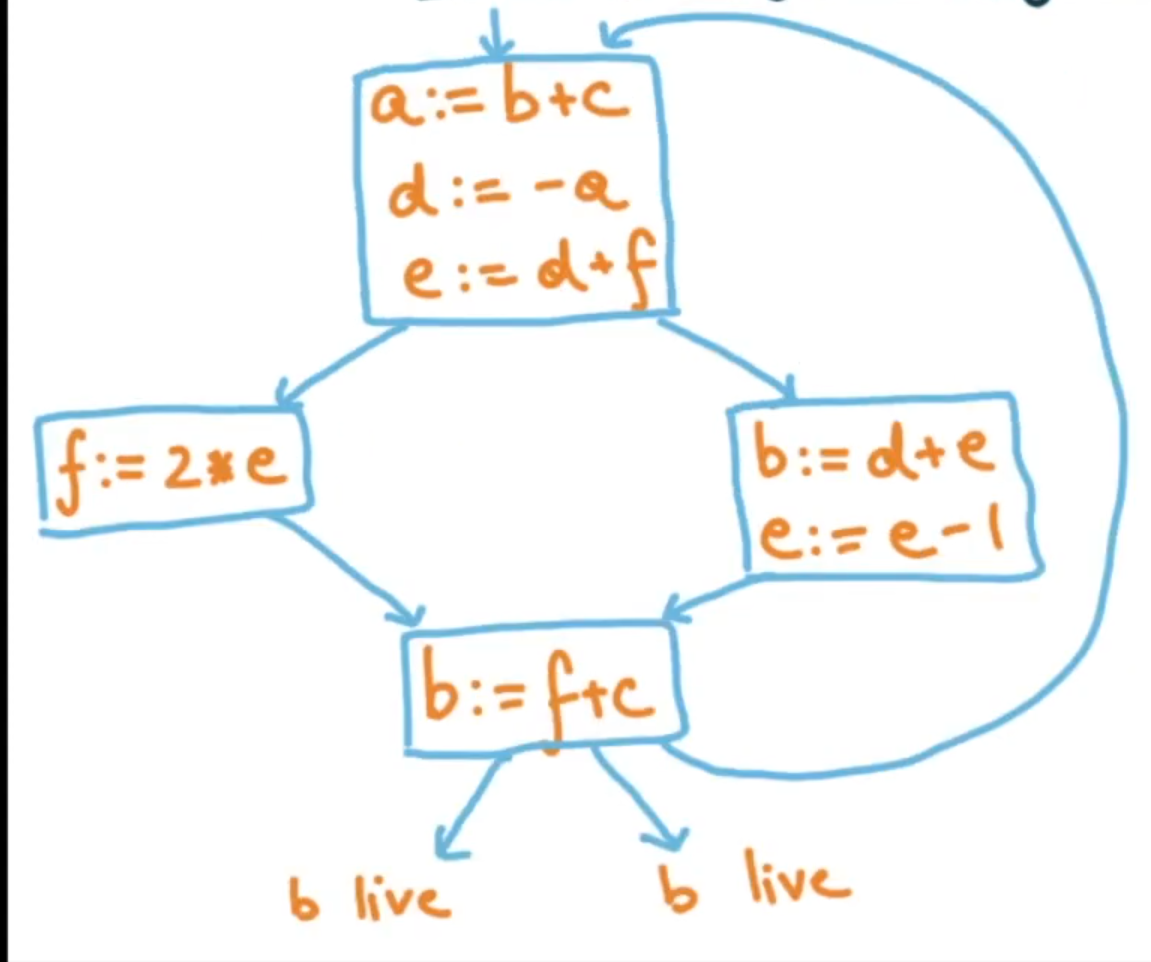
\includegraphics[scale=0.2]{images/85_eg.png}\\
The above image represents the control flow graph of the program under consideration.\\
Executing a liveness analysis on the program we get:\\
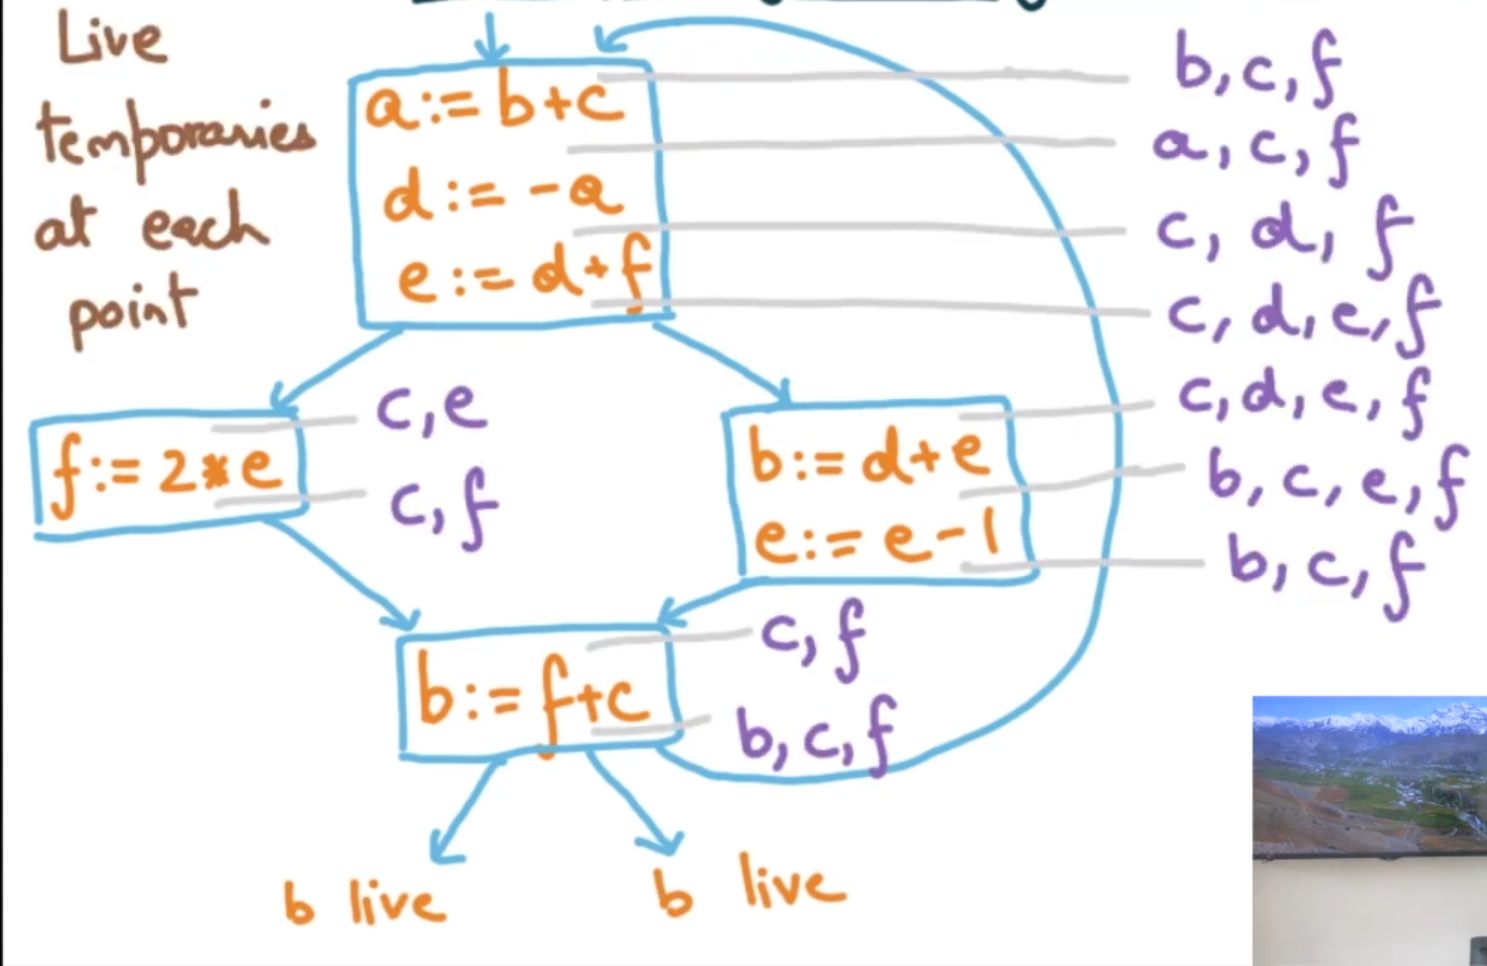
\includegraphics[scale=0.2]{images/85_eg2.png}\\
Everything in the purple pen represent the variables that are live at that particular program point.\\
Now we need to find the pairs of variables that are not live simultaneously at any program point. After going through the program points above, we see that the following pairs of variables are not live simultaneously.
\begin{itemize}
    \item (a,b)
    \item (b,d)
    \item (a,d)
    \item (a,e)
\end{itemize}
These pairs of variables can share a register. Moreover, from the pairs (a,b), (b,d), (a,d) we can infer that a,b,d can be allocated to the same register. \\
Next, we discuss an algorithm for register allocation from the ideas that we got from the two examples.
\subsection{Towards a Register Allocation Algorithm}
\begin{itemize}
    \item Construct an undirected graph.
    \item Node for every temporary
    \item There is an edge between t1 and t2 if they are simultaneously live at some program point.
    % \item Color the graph with k colors, where k is the number of registers. If this is possible we 
\end{itemize}


The undirected graph made is called as Register Interference Graph (RIG). If 2 temporaries do not have an edge between them then we can allocated them to the same register.\\
The RIG for the second example discussed above is\\
\begin{center}
    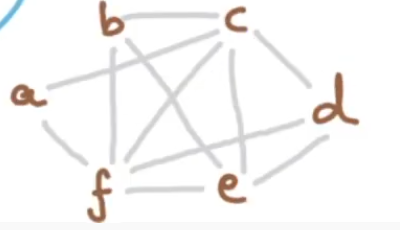
\includegraphics[scale=0.2]{images/85_RIGeg2.png}\\
\end{center}
As we can see that the RIG extracts a global picture from the program. Now we do not need to be concerned about any program point.\\
For any register allocation to be valid, any 2 temporaries mapped to the same register by the allocation must not have an edge between them.\\
% Motivated from this we can see Graph Coloring can help us in getting an allocation.\\
Lets just deviate and discuss a theoretical computer science problem.\\
\textbf{Graph Coloring:} An assignment of colours to each node of the graph so that nodes connected by an edge do not have the same color.\\
\textbf{k-colourable Graph:} A graph is k-colourable if it can be coloured with k colours.\\
On giving it a thought, we can see that the problem of graph colouring can help in validating if a register allocation is possible. Denote every register with a unique colour and try to colour the RIG with k colours, where k is the number of registers. If it is possible we get a valid register allocation for each temporary, else we need to spill some temporaries to memory.\\
% Unfortunately graph colouring is a NP hard problem. In the next module we discuss a heuristic based  